\documentclass[9pt]{pnas-new}
% Use the lineno option to display guide line numbers if required.
% Note that the use of elements such as single-column equations
% may affect the guide line number alignment. 

%\RequirePackage[english,slovene]{babel} % when writing in slovene
\RequirePackage[slovene,english]{babel} % when writing in english
\DeclareUnicodeCharacter{202F}{ }
\templatetype{pnasresearcharticle} % Choose template 
% {pnasresearcharticle} = Template for a two-column research article
% {pnasmathematics} = Template for a one-column mathematics article
% {pnasinvited} = Template for a PNAS invited submission
\usepackage{graphicx}
\usepackage{subcaption}
\usepackage{adjustbox}
\selectlanguage{english}
%\etal{in sod.} % comment out when writing in english
%\renewcommand{\Authands}{ in } % comment out when writing in english
%\renewcommand{\Authand}{ in } % comment out when writing in english

\newcommand{\set}[1]{\ensuremath{\mathbf{#1}}}
\renewcommand{\vec}[1]{\ensuremath{\mathbf{#1}}}
\newcommand{\uvec}[1]{\ensuremath{\hat{\vec{#1}}}}
\newcommand{\const}[1]{{\ensuremath{\kappa_\mathrm{#1}}}} 

\newcommand{\num}[1]{#1}

\graphicspath{{./fig/}}

\title{Swarming behaviour in predator-prey model}

% Use letters for affiliations, numbers to show equal authorship (if applicable) and to indicate the corresponding author
\author{Ariana Kržan}
\author{Tina Brdnik}
\author{Vito Levstik}

\affil{Collective behaviour course research seminar report} 

% Please give the surname of the lead author for the running footer
%\leadauthor{Lead author last name} 

\selectlanguage{english}

% Please add here a significance statement to explain the relevance of your work
\significancestatement{This research explores the emergence of collective behaviors in predator-prey dynamics using reinforcement learning
to simulate how survival pressures drive adaptive behaviors like swarming and evasion. 
By modeling multi-species interactions in a complex environment, the study extends current understanding of evolutionary survival strategies
and the role of learning in shaping group dynamics.}{Simulation | swarming behaviour | predator | prey}

\selectlanguage{english}

% Please include corresponding author, author contribution and author declaration information
%\authorcontributions{Please provide details of author contributions here.}
%\authordeclaration{Please declare any conflict of interest here.}
%\equalauthors{\textsuperscript{1}A.O.(Author One) and A.T. (Author Two) contributed equally to this work (remove if not applicable).}
%\correspondingauthor{\textsuperscript{2}To whom correspondence should be addressed. E-mail: author.two\@email.com}

% Keywords are not mandatory, but authors are strongly encouraged to provide them. If provided, please include two to five keywords, separated by the pipe symbol, e.g:
\keywords{Simulation | swarming behaviour | predator | prey} 

\begin{abstract}
    Collective animal behaviour, especially swarming in predator-prey dynamics, offers insights into survival strategies 
    that emerge under evolutionary pressures. This report outlines the initial objectives and foundational concepts for simulating 
    predator-prey. Inspired by previous work, we examine how survival pressures can drive emergent group behaviours
    in prey through reinforcement learning. We begin with an overview of related work, from classic rule-based models 
    to more recent reinforcement learning approaches, highlighting advances that allow agents to adapt to changing environments. 
    Our primary objective is to recreate a reinforcement learning-based model where predator-prey interactions lead to swarming 
    and evasion behaviours. The model will then extend to include environmental obstacles and an additional species, 
    enabling us to investigate the interplay between interspecies interactions and survival strategies. 
\end{abstract}

\dates{\textbf{\today}}
\program{BMA-RI}
\vol{2024/25}
\no{Group G} % group ID
%\fraca{FRIteza/201516.130}


\begin{document}

% Optional adjustment to line up main text (after abstract) of first page with line numbers, when using both lineno and twocolumn options.
% You should only change this length when you've finalised the article contents.
\verticaladjustment{-2pt}

\maketitle
\thispagestyle{firststyle}
\ifthenelse{\boolean{shortarticle}}{\ifthenelse{\boolean{singlecolumn}}{\abscontentformatted}{\abscontent}}{}

% If your first paragraph (i.e. with the \dropcap) contains a list environment (quote, quotation, theorem, definition, enumerate, itemize...), the line after the list may have some extra indentation. If this is the case, add \parshape=0 to the end of the list environment.
\dropcap{T}he sudden emergence of swarming behaviours in animals is one of the most striking examples of collective animal behaviour. 
These behaviours have been extensively studied for their implications for the evolution of cooperation, 
social cognition and predator–prey dynamics\cite{olson2013predator}. Swarming, which appears in many different species like starlings, 
herrings, and locusts, has been linked to several benefits including enhanced foraging efficiency, improved mating success, and distributed problem-solving abilities. 
Furthermore, they are hypothesized to help with improving group vigilance, reducing the chance of being encountered by predators, 
diluting an individual's risk of being attacked, enabling an active defence against predators and reducing predator attack efficiency by confusing the predator. \cite{li2023predator}.

In this project we will be taking inspiration from the work of Li et al. (2023) and Olson et al. (2013) to explore how survival pressures can drive the emergence of swarming behaviour. 
The first goal will be to create a realistic simulation where both prey and predators learn to adapt through reinforcement learning based on their drive to survive.
Modelling these interactions, we will observe how simple survival pressures can lead to evolution of more complex behaviours like flocking, swirling and edge predation. 

Then, we will extend our research by evolving out existing model by introducing new environmental obstacles and new species to observe how interspecies interactions lead to new survival strategies.

\section*{Related work}
The modelling of swarming behaviour has evolved from foundational rule-based frameworks to more sophisticated reinforcement learning (RL) approaches, with intermediate advances in topological and vision-based models that add realism to agent interactions.

\subsection{Rule-Based models}
Early models of swarming relied on static interaction rules to simulate basic group dynamics. 
Aoki's Zone Model (1982) introduced three interaction zones-repulsion, alignment, and attraction-where agents adjust their behaviour based on proximity to neighbours \cite{aoki1987zones}. 
Later, Vicsek's Model (1995) and Reynolds' Boids Model (1987) introduced basic alignment rules (and in Reynolds' case, also cohesion and separation) to generate coordinated group movement \cite{Vicsek1995}\cite{reynolds1987boids}. 
Although effective in modelling simple swarming behaviours, these models rely on fixed rules that limit agents' ability to adapt dynamically to changing environments or threats.

\subsection{Topological and Vision-Based Extensions}

Topological and vision-based models improved realism by adding sensory and neighbour-based constraints. 
Hemelrijk \& Hildenbrandt (2008) introduced a perception model where agents respond only to neighbours that are visible within a variable radius, adjusted by local density, stabilizing cohesion across varied densities \cite{Hemelrijk2008}. 
Kunz \& Hemelrijk (2012) further refined this approach by incorporating visual occlusion, where agents respond only to visible neighbours, simulating real-world sensory limitations \cite{kunz2012}. While these models increase biological realism, they remain rule-based and lack the flexibility of adaptive RL models.

\subsection{Learning-Based Models}

Learning-based approaches have enabled significant advances in modeling swarming behaviors, allowing agents to develop adaptive strategies based on interactions rather than fixed rules. These models often produce dynamic, emergent behaviors such as flocking and evasion, closely mimicking natural adaptive responses to survival pressures.

\begin{itemize}
    \item Olson et al. (2013): Olson and colleagues used a genetic algorithm (GA) to model predator confusion, where prey evolved to cluster and thereby reduce individual predation risk by confusing predators \cite{olson2013predator}. This GA-based approach demonstrates the power of evolutionary adaptation in fostering emergent clustering behaviors in predator-prey dynamics.
    \item Lowe et al. (2017): The Multi-Agent Deep Deterministic Policy Gradient (MADDPG) algorithm enables agents to learn in mixed cooperative and competitive environments, making it ideal for systems with multiple interacting species \cite{lowe2017}. MADDPG is a reinforcement learning method that combines centralized training (using global information for critics) with decentralized execution (using local observations for policies). It supports complex, dynamic environments by allowing agents to optimize strategies in both cooperative and adversarial contexts, such as predators and prey with differing objectives.
    \item Li et al. (2023): In this RL-based predator-prey model, prey agents develop swarming behaviors by maximizing survival rewards and minimizing capture penalties \cite{li2023predator}. Prey adaptively form cohesive groups and evade predators, learning these behaviors through experience rather than pre-set alignment rules.
\end{itemize}


\section*{Methods}

Our proposed methodology aims to simulate swarming behaviours in a predator-prey environment using reinforcement learning (RL). 
We will define and test a RL-based model where agents, such as prey and predators interact within a two-dimensional space. The goal is to observe how different pressures and interactions influence collective behaviours like swarming, evasion, and strategic movement.

\subsection{Environment Setup}
The simulation will take place in a 2D environment with open and confined spaces. The confined space will have stiff boundaries, meaning
that agents will bounce off them when they collide, whereas the open space will have periodic boundaries, meaning that agents will reappear on the opposite side when they cross the boundary.
Such setup with periodic boundaries serves as an approximation of an infinite space, allowing agents to move freely without encountering physical borders. 
Later on, we wish to place random obstacles, which will be distributed across the space to create a complex and realistic setting that challenges the agents to adapt their movement and coordination. 

We will apply the perception and action models from Li et al. (2023) \cite{li2023predator} to guide agent interactions in the simulation.

\begin{itemize}
    \item \textbf{Perception Model}: Each agent detects others only within a specified range and limited to a maximum number of nearby agents, simulating real-world sensory limitations.
    \item \textbf{Action Model}: Agents adjust their movement through forward propulsion and directional changes, governed by RL policies that optimize goals like survival and prey capture.
\end{itemize}

\subsection{Agent Types and Behaviour}
\begin{itemize}
    \item \textbf{Prey}: These agents aim to survive by avoiding predators and moving as a group.
    \item \textbf{Predators}: Predators are designed to pursue and catch prey.
    \item \textbf{New Species}: We may introduce a third type of agent, such as a neutral species, scavenger or competitor, which will have its own survival or resource-based objectives.
\end{itemize}

\subsection{Reinforcement Learning Framework}
\begin{itemize}
    \item \textbf{Algorithm}: We plan to use the Multi-Agent Deep Deterministic Policy Gradient (MADDPG) algorithm.
    \item \textbf{Reward Structure}:
        \begin{itemize}
            \item \textbf{Prey}: Rewarded for survival over time, with penalties for being caught.
            \item \textbf{Predators}: Rewarded for capturing prey, with penalties for colliding with obstacles.
            \item \textbf{New Species}: Rewarded based on interactions like resource competition or cooperation with other agents.
        \end{itemize}
    \item \textbf{Training Setup}: Agents will be trained through episodic simulations, allowing them to learn and adapt from each episode's interactions. We will vary conditions to observe how changes influence learned behaviours.
\end{itemize}

\subsection*{Proposed Methodology for Verification}

To verify the behavior of our model, we will adopt the methodology described in Li et al. (2023) \cite{li2023predator}, utilizing two key metrics: the Degree of Alignment (DoA) and the Degree of Separation (DoS).

\begin{itemize}
    \item \textbf{Degree of Sparsity (DoS):} This metric measures the spatial aggregation of agents, capturing how densely the agents cluster together. It is defined as:
    \[
    \text{DoS} = \frac{1}{TND} \sum_{t=1}^T \sum_{j=1}^N \| \mathbf{x}_j(t) - \mathbf{x}_k(t) \|
    \]
    where: \( \mathbf{x}_j(t) \) is the position of the \(j\)-th agent at time step \(t\), \( \mathbf{x}_k(t) \) is the position of the nearest neighbor \(k = \arg\min_k \| \mathbf{x}_j(t) - \mathbf{x}_k(t) \| \), \(T\) is the episode length, \(N\) is the total number of agents, and \(D\) is the maximum possible distance between two agents in the environment.
    
    A smaller DoS value indicates denser clustering, while a value of 0 represents all agents aggregating at a single point.

    \item \textbf{Degree of Alignment (DoA):} This metric quantifies the alignment of the agents' headings, assessing how consistently agents move in the same direction. It is defined as:
    \[
    \text{DoA} = \frac{1}{2TN} \sum_{t=1}^T \sum_{j=1}^N \| \mathbf{h}_j(t) + \mathbf{h}_k(t) \|
    \]
    where: \( \mathbf{h}_j(t) \) is the heading of the \(j\)-th agent at time step \(t\), \( \mathbf{h}_k(t) \) is the heading of the nearest neighbor of agent \(j\) (the same nearest neighbor as in the DoS calculation), \(T\) is the episode length, and \(N\) is the total number of agents.
    
    Higher DoA values indicate stronger alignment in agent movement. It is important to note that the DoA measures local alignment between neighboring agents rather than the mean heading of the entire group, making it more suitable for detecting relative alignment within swarms.
\end{itemize}

By analyzing these metrics during and after training, we aim to verify whether our model reproduces swarming behaviors.


\section*{Results}

In the initial phase of our project, we implemented a basic model in an environment with periodic borders and agents controlled by passive and active forces. 
In this part of the project these forces were initialized with random values for the activity parameters $a_f$ and $a_r$, which we planned to optimize using reinforcement learning (RL). 
The $a_f$ component controls the agent's forward movement, aligned with its current heading, while the $a_r$ component adjusts the agent's heading through rotational actions.
The agents followed a reward-based decision-making system, designed to maximize survival and promote swarming behaviors similar to those described in Li et al. (2023).

We initially attempted to develop our own RL model to train the activity parameters $a_f$ and $a_r$, but the results were unsatisfactory. 
Instead of achieving complex swarming behaviors, the agents displayed repetitive circular motions that failed to maximize rewards or encourage meaningful group dynamics. 

\begin{figure}[ht]
	\centering
	% Subfigure (a)
	\begin{subfigure}{0.30\textwidth}
		\centering
		\fbox{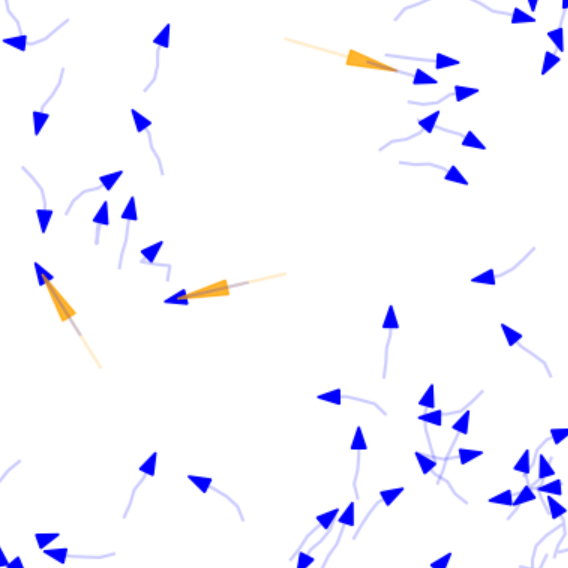
\includegraphics[width=\textwidth]{fig/reward.png}}
		\vspace{0.5em}
		\centering (a)
	\end{subfigure}
	\hfill
	% Subfigure (b)
	\begin{subfigure}{0.30\textwidth}
		\centering
		\fbox{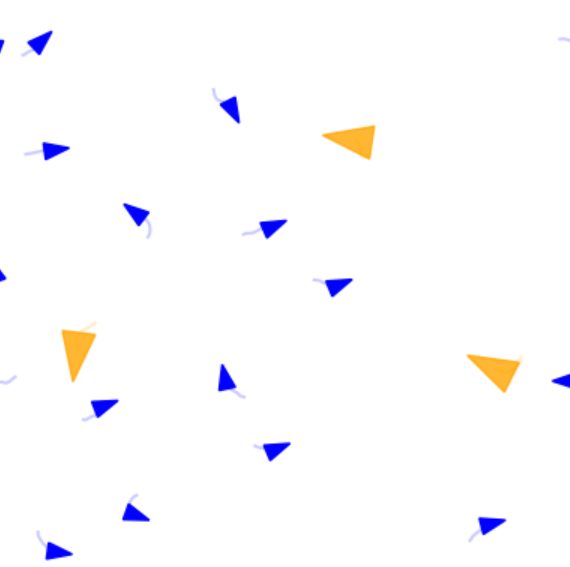
\includegraphics[width=\textwidth]{fig/basic2.png}}
		\vspace{0.5em}
		\centering (b)
	\end{subfigure}
	\hfill
	% Subfigure (c)
	\begin{subfigure}{0.30\textwidth}
		\centering
		\fbox{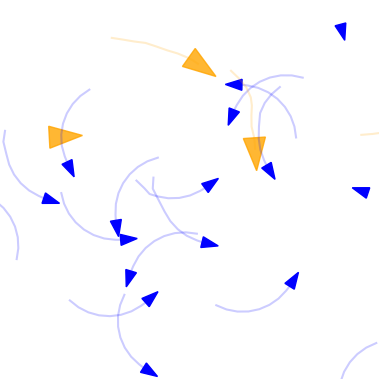
\includegraphics[width=\textwidth]{fig/withRL.png}}
		\vspace{0.5em}
		\centering (c)
	\end{subfigure}
	
	\caption{(a) Our model with no RL component, following the reward system. (b) Our model with no RL component, with random initialization of parameters (c) Our model with RL.}
	\label{fig:three_images}
\end{figure}

Recognizing these limitations, we decided to adopt the RL model from the Li et al. article \cite{li2023predator}.
Using their code, we were able to successfully run simulations of their model in our environment. 
This provided a functioning baseline for comparison and further experimentation.
Preliminary results from this approach, however, did not fully replicate the swarming behaviors reported in their study.
Our results show significant variability in both the Degree of Separation (DoS) and Degree of Alignment (DoA) across episodes, with no clear trends indicating improvement. 
The fluctuating DoS suggests that agents fail to form stable clusters, while the inconsistent DoA values indicate a lack of coordinated alignment among agents. 
These results suggest that the model has not converged effectively, likely due to issues with the reward structure or suboptimal parameter tuning. 
Further refinement is needed to achieve consistent swarming behaviors.

\begin{figure}[htbp]
    \centering
    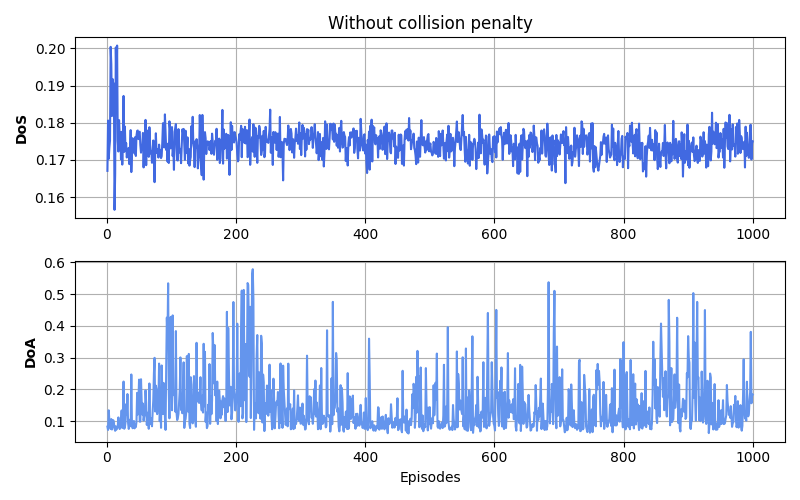
\includegraphics[width=0.7\textwidth]{fig/Without_collision.png}
    \caption{Degree of Alignment (DoA) and Degree of Separation (DoS) across episodes without collision penalty. The DoA remains highly variable, while the DoS shows no clear clustering trend.}
    \label{fig:doa_dos_without_collision}
\end{figure}


\section*{Discussion}
In this stage of the project, we successfully ran the code from the main article but encountered challenges with the agents' behavior. 
The DoA and DoS metrics remain highly variable, indicating that swarming behaviors have not yet emerged. 
These results suggest the need for further tuning of the reward structure and additional training.

Despite the setbacks, we are motivated to continue refining the model and addressing these issues. 
Our next steps are to improve the code to produce results similar to the article, introduce obstacles to the environment, and add a new species, which we have yet to finalize.

\acknow{AK worked on models with and without RL component implementations, TB worked on graphs, methods, results and discussion, VL worked on .}
\showacknow % Display the acknowledgments section

% \pnasbreak splits and balances the columns before the references.
% If you see unexpected formatting errors, try commenting out this line
% as it can run into problems with floats and footnotes on the final page.
%\pnasbreak

\begin{multicols}{2}
	%\bibliographystyle{plain} % or any style you prefer, such as ieee, unsrt, etc.
	\bibliography{bib/bibliography} % This assumes your .bib file is located at ./bib/bibliography.bib
\end{multicols}


\end{document}
